% Options for packages loaded elsewhere
\PassOptionsToPackage{unicode}{hyperref}
\PassOptionsToPackage{hyphens}{url}
\documentclass[
  ignorenonframetext,
]{beamer}
\newif\ifbibliography
\usepackage{pgfpages}
\setbeamertemplate{caption}[numbered]
\setbeamertemplate{caption label separator}{: }
\setbeamercolor{caption name}{fg=normal text.fg}
\beamertemplatenavigationsymbolsempty
% remove section numbering
\setbeamertemplate{part page}{
  \centering
  \begin{beamercolorbox}[sep=16pt,center]{part title}
    \usebeamerfont{part title}\insertpart\par
  \end{beamercolorbox}
}
\setbeamertemplate{section page}{
  \centering
  \begin{beamercolorbox}[sep=12pt,center]{section title}
    \usebeamerfont{section title}\insertsection\par
  \end{beamercolorbox}
}
\setbeamertemplate{subsection page}{
  \centering
  \begin{beamercolorbox}[sep=8pt,center]{subsection title}
    \usebeamerfont{subsection title}\insertsubsection\par
  \end{beamercolorbox}
}
% Prevent slide breaks in the middle of a paragraph
\widowpenalties 1 10000
\raggedbottom
\AtBeginPart{
  \frame{\partpage}
}
\AtBeginSection{
  \ifbibliography
  \else
    \frame{\sectionpage}
  \fi
}
\AtBeginSubsection{
  \frame{\subsectionpage}
}
\usepackage{iftex}
\ifPDFTeX
  \usepackage[T1]{fontenc}
  \usepackage[utf8]{inputenc}
  \usepackage{textcomp} % provide euro and other symbols
\else % if luatex or xetex
  \usepackage{unicode-math} % this also loads fontspec
  \defaultfontfeatures{Scale=MatchLowercase}
  \defaultfontfeatures[\rmfamily]{Ligatures=TeX,Scale=1}
\fi
\usepackage{lmodern}
\ifPDFTeX\else
  % xetex/luatex font selection
\fi
% Use upquote if available, for straight quotes in verbatim environments
\IfFileExists{upquote.sty}{\usepackage{upquote}}{}
\IfFileExists{microtype.sty}{% use microtype if available
  \usepackage[]{microtype}
  \UseMicrotypeSet[protrusion]{basicmath} % disable protrusion for tt fonts
}{}
\makeatletter
\@ifundefined{KOMAClassName}{% if non-KOMA class
  \IfFileExists{parskip.sty}{%
    \usepackage{parskip}
  }{% else
    \setlength{\parindent}{0pt}
    \setlength{\parskip}{6pt plus 2pt minus 1pt}}
}{% if KOMA class
  \KOMAoptions{parskip=half}}
\makeatother
\usepackage{longtable,booktabs,array}
\usepackage{caption}
\captionsetup[table]{skip=6pt}
\newcounter{none} % for unnumbered tables
\usepackage{calc} % for calculating minipage widths
\usepackage{caption}
% Make caption package work with longtable
\makeatletter
\def\fnum@table{\tablename~\thetable}
\makeatother
\usepackage{graphicx}
\makeatletter
\newsavebox\pandoc@box
\newcommand*\pandocbounded[1]{% scales image to fit in text height/width
  \sbox\pandoc@box{#1}%
  \Gscale@div\@tempa{\textheight}{\dimexpr\ht\pandoc@box+\dp\pandoc@box\relax}%
  \Gscale@div\@tempb{\linewidth}{\wd\pandoc@box}%
  \ifdim\@tempb\p@<\@tempa\p@\let\@tempa\@tempb\fi% select the smaller of both
  \ifdim\@tempa\p@<\p@\scalebox{\@tempa}{\usebox\pandoc@box}%
  \else\usebox{\pandoc@box}%
  \fi%
}
% Set default figure placement to htbp
\def\fps@figure{htbp}
\makeatother
\setlength{\emergencystretch}{3em} % prevent overfull lines
\providecommand{\tightlist}{%
  \setlength{\itemsep}{0pt}\setlength{\parskip}{0pt}}
% Manuscript macro/package fallbacks (newcommand -> providecommand).
\usepackage{amsmath}
\usepackage{amssymb}
\usepackage{booktabs}
% Contents listing: article.cls prefixes every \l@section entry with
% \addvspace{1.0em}, which across ten sections costs about ten lines and pushed
% the ~40-entry listing one line past page 2 — leaving a third sheet carrying a
% single "10 References" line. Tighten that inter-section gap for the duration
% of \tableofcontents only, inside a group, so body spacing is untouched and no
% entry is dropped (reducing \tocdepth would have hidden 29 real subsections).
  \providecommand{\addvspace}[1]{\vskip 2\p@}%
% Document metadata. config.yaml declares a subtitle and a keyword list, and
% the producer emits both as tokens, but the template's \hypersetup writes only
% pdftitle/pdfauthor/pdflang -- so `pdfinfo` reported no Subject and no
% Keywords. This block runs after the template's, so it wins.
%
% The two values below are WRITTEN by scripts/z_generate_manuscript_variables.py
% (sync_preamble_metadata), never typed. A double-brace token cannot be used here:
% preamble.md is substituted into output/manuscript/ like any other section, but
% the template's _manuscript_source.py then copies the raw file back over that
% copy, so an unresolved token would reach hyperref and land in the PDF's
% metadata verbatim.
% Bounded identifier splitting. The template defines
%   \protected\def\breaktt#1{\begingroup\ttfamily\seqsplit{#1}\endgroup}
% and \seqsplit permits a break after EVERY character with no continuation cue.
% In the 2026-09-05 PDF that rendered `model_family_manifest.json` as
% `model_family_manifest.js` + `on` and `src/manuscript_variables.py` as
% `(src/manusc` + `ript_variables.py` — the first is itself a valid filename, so
% a reader cannot tell a line break from a name. Keep seqsplit's guarantee that
% no code token overflows the measure, but forbid breaks inside the last
% \GNNttTail characters (an extension is never orphaned) and inside the first
% \GNNttHead (a one- or two-letter stub is never left behind).
% Declarations the template's combined-PDF renderer requires
% (infrastructure/rendering/_pdf_combined_preamble.py). Absent here, it warns
% "Preamble is missing declarations required by manuscript content" and
% appends these exact lines itself; declaring them explicitly silences the
% warning without changing the typeset document.
\usepackage{listings}
\lstset{basicstyle=\ttfamily\small,breaklines=true,columns=fullflexible}

\usepackage{fvextra}
\fvset{breaklines=true,breakanywhere=true,breaknonspaceingroup=true,breaksymbolleft={},breaksymbolright={},breakanywheresymbolpre={},breakanywheresymbolpost={}}
\RecustomVerbatimEnvironment{verbatim}{Verbatim}{}

\makeatletter
\newbox\archive@titlebox
\newdimen\archive@available
\newcommand*\archivefigurebounded[1]{%
  \sbox\pandoc@box{#1}%
  \archive@available=\textheight%
  \ifx\beamer@frametitle\@empty\else%
    \setbox\archive@titlebox=\vbox{\vbox{}{\parskip0pt\usebeamertemplate***{frametitle}\vskip0.25em}}%
    \advance\archive@available by-\ht\archive@titlebox%
    \advance\archive@available by-\dp\archive@titlebox%
  \fi%
  \advance\archive@available by-\beamer@frametopskip%
  \advance\archive@available by-2\baselineskip%
  \ifdim\archive@available<1pt%
    \PackageError{template}{Archive image frame has no title-safe image area}{}%
  \fi%
  \Gscale@div\@tempa{\archive@available}{\dimexpr\ht\pandoc@box+\dp\pandoc@box\relax}%
  \Gscale@div\@tempb{0.98\linewidth}{\wd\pandoc@box}%
  \ifdim\@tempb\p@<\@tempa\p@\let\@tempa\@tempb\fi%
  \ifdim\@tempa\p@<\p@\scalebox{\@tempa}{\usebox\pandoc@box}%
  \else\usebox{\pandoc@box}\fi%
}
\newcommand*\archivefigurecaptionnumber[2]{#2}
\newenvironment{archivecaptionframe}{\par\begingroup}{\par\endgroup}
\newenvironment{archiveimageframe}{\par\begingroup\centering\let\pandocbounded\archivefigurebounded}{\par\endgroup}
\ifdefined\pandocbounded
\renewcommand*\pandocbounded[1]{%
  \sbox\pandoc@box{#1}%
  \Gscale@div\@tempa{0.40\textheight}{\dimexpr\ht\pandoc@box+\dp\pandoc@box\relax}%
  \Gscale@div\@tempb{0.98\linewidth}{\wd\pandoc@box}%
  \ifdim\@tempb\p@<\@tempa\p@\let\@tempa\@tempb\fi%
  \ifdim\@tempa\p@<\p@\scalebox{\@tempa}{\usebox\pandoc@box}%
  \else\usebox{\pandoc@box}%
  \fi%
}
\fi
\makeatother

% Slide layout defaults for warning-clean scientific decks.
\usepackage{etoolbox}
\IfFileExists{xurl.sty}{\usepackage{xurl}}{}
\IfFileExists{seqsplit.sty}{\usepackage{seqsplit}}{}
\providecommand{\seqsplit}[1]{#1}
\protected\def\breakseq#1{\seqsplit{#1}}
\protected\def\breaktt#1{\begingroup\ttfamily\seqsplit{#1}\endgroup}
\setlength{\emergencystretch}{6em}
\tolerance=5000
\hbadness=10000
\hfuzz=1pt
\setlength{\tabcolsep}{2pt}
\AtBeginEnvironment{longtable}{\tiny\renewcommand{\arraystretch}{0.86}\setlength{\tabcolsep}{1pt}}
\AtBeginEnvironment{tabular}{\tiny\renewcommand{\arraystretch}{0.86}\setlength{\tabcolsep}{1pt}}
\AtBeginEnvironment{equation}{\tiny}
\AtBeginEnvironment{equation*}{\tiny}
\AtBeginEnvironment{align}{\tiny}
\AtBeginEnvironment{align*}{\tiny}
\AtBeginEnvironment{itemize}{\footnotesize}
\AtBeginEnvironment{enumerate}{\footnotesize}
\AtBeginEnvironment{description}{\footnotesize}
\setbeamerfont{caption}{size=\tiny}
\setbeamerfont{caption name}{size=\tiny}
\setbeamerfont{normal text}{size=\small}
\setbeamerfont{frametitle}{size=\small}
\setbeamerfont{section title}{size=\footnotesize}
\setbeamerfont{subsection title}{size=\footnotesize}
\setbeamertemplate{section page}{%
  \centering
  \begin{beamercolorbox}[sep=12pt,center,wd=\paperwidth]{section title}
    \parbox{0.86\paperwidth}{\centering\usebeamerfont{section title}\insertsection\par}
  \end{beamercolorbox}
}
\setbeamertemplate{subsection page}{%
  \centering
  \begin{beamercolorbox}[sep=8pt,center,wd=\paperwidth]{subsection title}
    \parbox{0.86\paperwidth}{\centering\usebeamerfont{subsection title}\insertsubsection\par}
  \end{beamercolorbox}
}
\setlength{\abovecaptionskip}{2pt}
\setlength{\belowcaptionskip}{0pt}

% Natbib and cross-reference fallbacks — slides don't load natbib
% or cleveref, but combined-PDF manuscript prose may emit these
% commands. The fallback renders citations as a bracketed key list
% and cross-references as detokenized labels so slides don't fail on
% undefined control sequences or raw underscores. \providecommand is
% a no-op if packages load later.
\providecommand{\citep}[1]{[#1]}
\providecommand{\citet}[1]{#1}
\providecommand{\citealp}[1]{#1}
\providecommand{\citeauthor}[1]{#1}
\providecommand{\citeyear}[1]{#1}
\providecommand{\cref}[1]{\texttt{\detokenize{#1}}}
\providecommand{\Cref}[1]{\texttt{\detokenize{#1}}}
\providecommand{\crefrange}[2]{\texttt{\detokenize{#1}}--\texttt{\detokenize{#2}}}
\providecommand{\Crefrange}[2]{\texttt{\detokenize{#1}}--\texttt{\detokenize{#2}}}
\providecommand{\paragraph}[1]{\textbf{#1}\ }

\newtheorem{proposition}{Proposition}
\newtheorem{hypothesis}{Hypothesis}
\newtheorem{remark}[theorem]{Remark}
\newtheorem{axiom}{Axiom}
\newtheorem{property}{Property}
\usepackage{bookmark}
\IfFileExists{xurl.sty}{\usepackage{xurl}}{} % add URL line breaks if available
\urlstyle{same}
% fallback for those not using the hyperref driver hyperxmp:
\makeatletter
\@ifundefined{xmpquote}{\newcommand{\xmpquote}[1]{#1}}{}
\makeatother
\hypersetup{
  hidelinks,
  pdfcreator={LaTeX via pandoc}}

\author{\texorpdfstring{}{}}
\date{}

\begin{document}

\section{Artifacts and Evidence}\label{sec:artifacts_evidence}

\begin{frame}[allowframebreaks]{Artifacts and Evidence}
This section reports what the project has actually produced and how each
quantitative claim is grounded. Every number below is substituted at
render time from the deterministic producer, which reads the repository
state at commit 11a696d6e, so each figure here is regenerated from the
artifacts it describes rather than transcribed.
\end{frame}

\begin{frame}[fragile,allowframebreaks]{Model-Family Coverage}
\protect\phantomsection\label{model-family-coverage}
GNN ships a curated corpus of model families that exercise the language
across the difficulty gradient from minimal parser fixtures to full
multi-agent and scaling studies. The manifest registers 9 families
(basics, discrete, continuous, hierarchical, multiagent, precision,
structured, gridworld, scaling-study) across 9 target directories, and
\texttt{input/gnn\_files} holds 12 corpus directories containing 38
concrete example models. The three sets are not coextensive, and the
manuscript does not treat them as one. Registered in no family:
\breaktt{input/gnn\_files/learning}, \breaktt{input/gnn\_files/recursive},
\breaktt{input/gnn\_files/thrml} (3 of the 12 corpus directories),
covered in sec.~7. Registered but outside
the scanned tree: none, because all 9 target directories are themselves
\texttt{input/gnn\_files} corpus directories. Each family declares the
simulation frameworks it is meant to drive, which is what lets the same
\end{frame}

\begin{frame}[fragile,allowframebreaks]{Model-Family Coverage}
text model fan out across the executable-model leg of the Triple Play
(Smékal and Friedman 2023). The families and their declared frameworks
are enumerated below.

The exemplar corpus partitions cleanly by model kind, and the partition
is itself a token: 29 of the 38 example specifications are
discrete-state --- the discrete categorical kind and its composed
variants --- and 9 are continuous linear-Gaussian specifications in the
continuous family folder. The cold-start index
\breaktt{input/gnn\_files/INDEX.md} catalogues every exemplar with its
kind, its task folder, and a suggested reading order, and is the fastest
surface for a reader who wants to move from this prose to a runnable
file of a given kind.

\end{frame}

\begin{frame}[fragile,allowframebreaks]{Model-Family Coverage}
Families that declare a capability axis (the continuous family declares
the continuous-render axis) carry a backend split in
tbl.~\ref{tbl:model_families} generated directly from the registry's
declared capability flags. This avoids a manually copied registry table;
actual model admission still depends on the full parameter and
composition checks recorded by the renderer. The generated flags
describe declared capability, while current-run receipts record which
selected backends were actually attempted, unsupported, skipped, or
failed. The profiled cross-framework reference uses the continuous
family, so it does not establish categorical coverage across the
registry (tbl.~4 is the per-kind key).

\end{frame}

\begin{frame}[fragile,allowframebreaks]{Model-Family Coverage}
\begin{longtable}[]{@{}
  >{\raggedright\arraybackslash}p{(\linewidth - 4\tabcolsep) * \real{0.3333}}
  >{\raggedright\arraybackslash}p{(\linewidth - 4\tabcolsep) * \real{0.3333}}
  >{\raggedright\arraybackslash}p{(\linewidth - 4\tabcolsep) * \real{0.3333}}@{}}
\caption{Model families declared in
\protect\breaktt{input/model\_family\_manifest.json} with the simulation
frameworks each family targets and a generated description. The
\emph{Frameworks} column is the family's declared targets, verbatim from
the manifest; the capability splits appended to some descriptions are
generated from \protect\breaktt{src/gnn/render/framework\_registry.py}
flags, not authored in the manifest, so they cannot disagree with the
registry. Read with tbl.~3 (what each backend
is) and fig.~6 (the same coverage as a
matrix).}\label{tbl:model_families}\tabularnewline
\toprule\noalign{}
\begin{minipage}[b]{\linewidth}\raggedright
F\allowbreak{}a\allowbreak{}m\allowbreak{}i\allowbreak{}l\allowbreak{}y
\end{minipage} & \begin{minipage}[b]{\linewidth}\raggedright
F\allowbreak{}r\allowbreak{}a\allowbreak{}m\allowbreak{}e\allowbreak{}w\allowbreak{}o\allowbreak{}r\allowbreak{}k\allowbreak{}s
\end{minipage} & \begin{minipage}[b]{\linewidth}\raggedright
D\allowbreak{}e\allowbreak{}s\allowbreak{}c\allowbreak{}r\allowbreak{}i\allowbreak{}p\allowbreak{}t\allowbreak{}i\allowbreak{}o\allowbreak{}n
\end{minipage} \\
\midrule\noalign{}
\endfirsthead
\toprule\noalign{}
\begin{minipage}[b]{\linewidth}\raggedright
F\allowbreak{}a\allowbreak{}m\allowbreak{}i\allowbreak{}l\allowbreak{}y
\end{minipage} & \begin{minipage}[b]{\linewidth}\raggedright
F\allowbreak{}r\allowbreak{}a\allowbreak{}m\allowbreak{}e\allowbreak{}w\allowbreak{}o\allowbreak{}r\allowbreak{}k\allowbreak{}s
\end{minipage} & \begin{minipage}[b]{\linewidth}\raggedright
D\allowbreak{}e\allowbreak{}s\allowbreak{}c\allowbreak{}r\allowbreak{}i\allowbreak{}p\allowbreak{}t\allowbreak{}i\allowbreak{}o\allowbreak{}n
\end{minipage} \\
\midrule\noalign{}
\endhead
\texttt{basics} & pymdp & Minimal perception fixtures used for parser
and validator smoke coverage. \\
\texttt{discrete} & pymdp, jax & Discrete POMDP, passive HMM filtering
and episodic contingent T-maze fixtures. \\
\texttt{continuous} & jax, numpyro, stan, rxinfer, ngclearn &
Continuous-state linear-Gaussian fixtures (F/H/Q/R + Gaussian prior;
continuous\_navigation closes the loop on beliefs; ngc-learn LGSSM
exemplar for the ngclearn backend). Native on RxInfer.jl, JAX, PyTorch,
NumPyro, Stan, cpomdp, ngc-learn; reported unsupported (not failed) on
PyMDP, ActiveInference.jl, DisCoPy, bnlearn, THRML. \\
\texttt{hierarchical} & jax & Declared block-reset hierarchy and
approximate 10/100-clock soft-message controller fixtures. \\
\texttt{multiagent} & rxinfer & Multi-agent coordination and swarm
fixtures. \\
\texttt{precision} & pymdp & Precision weighting and curiosity-driven
fixtures. \\
\texttt{structured} & pymdp & Structured factor graph and posterior
fixtures. \\
\texttt{gridworld} & pymdp, rxinfer, activeinference\_jl & Gridworld
POMDP fixture used for cross-framework acceptance checks. \\
\bottomrule\noalign{}
\end{longtable}

\end{frame}

\begin{frame}[fragile,allowframebreaks]{Model-Family Coverage}

{\def\LTcaptype{none} % do not increment counter
\begin{longtable}[]{@{}
  >{\raggedright\arraybackslash}p{(\linewidth - 4\tabcolsep) * \real{0.3333}}
  >{\raggedright\arraybackslash}p{(\linewidth - 4\tabcolsep) * \real{0.3333}}
  >{\raggedright\arraybackslash}p{(\linewidth - 4\tabcolsep) * \real{0.3333}}@{}}
\toprule\noalign{}
\begin{minipage}[b]{\linewidth}\raggedright
F\allowbreak{}a\allowbreak{}m\allowbreak{}i\allowbreak{}l\allowbreak{}y
\end{minipage} & \begin{minipage}[b]{\linewidth}\raggedright
F\allowbreak{}r\allowbreak{}a\allowbreak{}m\allowbreak{}e\allowbreak{}w\allowbreak{}o\allowbreak{}r\allowbreak{}k\allowbreak{}s
\end{minipage} & \begin{minipage}[b]{\linewidth}\raggedright
D\allowbreak{}e\allowbreak{}s\allowbreak{}c\allowbreak{}r\allowbreak{}i\allowbreak{}p\allowbreak{}t\allowbreak{}i\allowbreak{}o\allowbreak{}n
\end{minipage} \\
\midrule\noalign{}
\endhead
\texttt{scaling-study} & pymdp & PyMDP scaling-study fixtures, sampled
conservatively for acceptance. \\
\bottomrule\noalign{}
\end{longtable}
}

\end{frame}

\begin{frame}[fragile,allowframebreaks]{Model-Family Coverage}
The family-by-framework structure is shown in
fig.~6, which renders the coverage matrix directly
from the family registry rather than from a hand-maintained table.

\end{frame}

\begin{frame}[fragile,allowframebreaks]{Model-Family Coverage}

\refstepcounter{figure}\label{fig:family_matrix}

\begin{archiveimageframe}

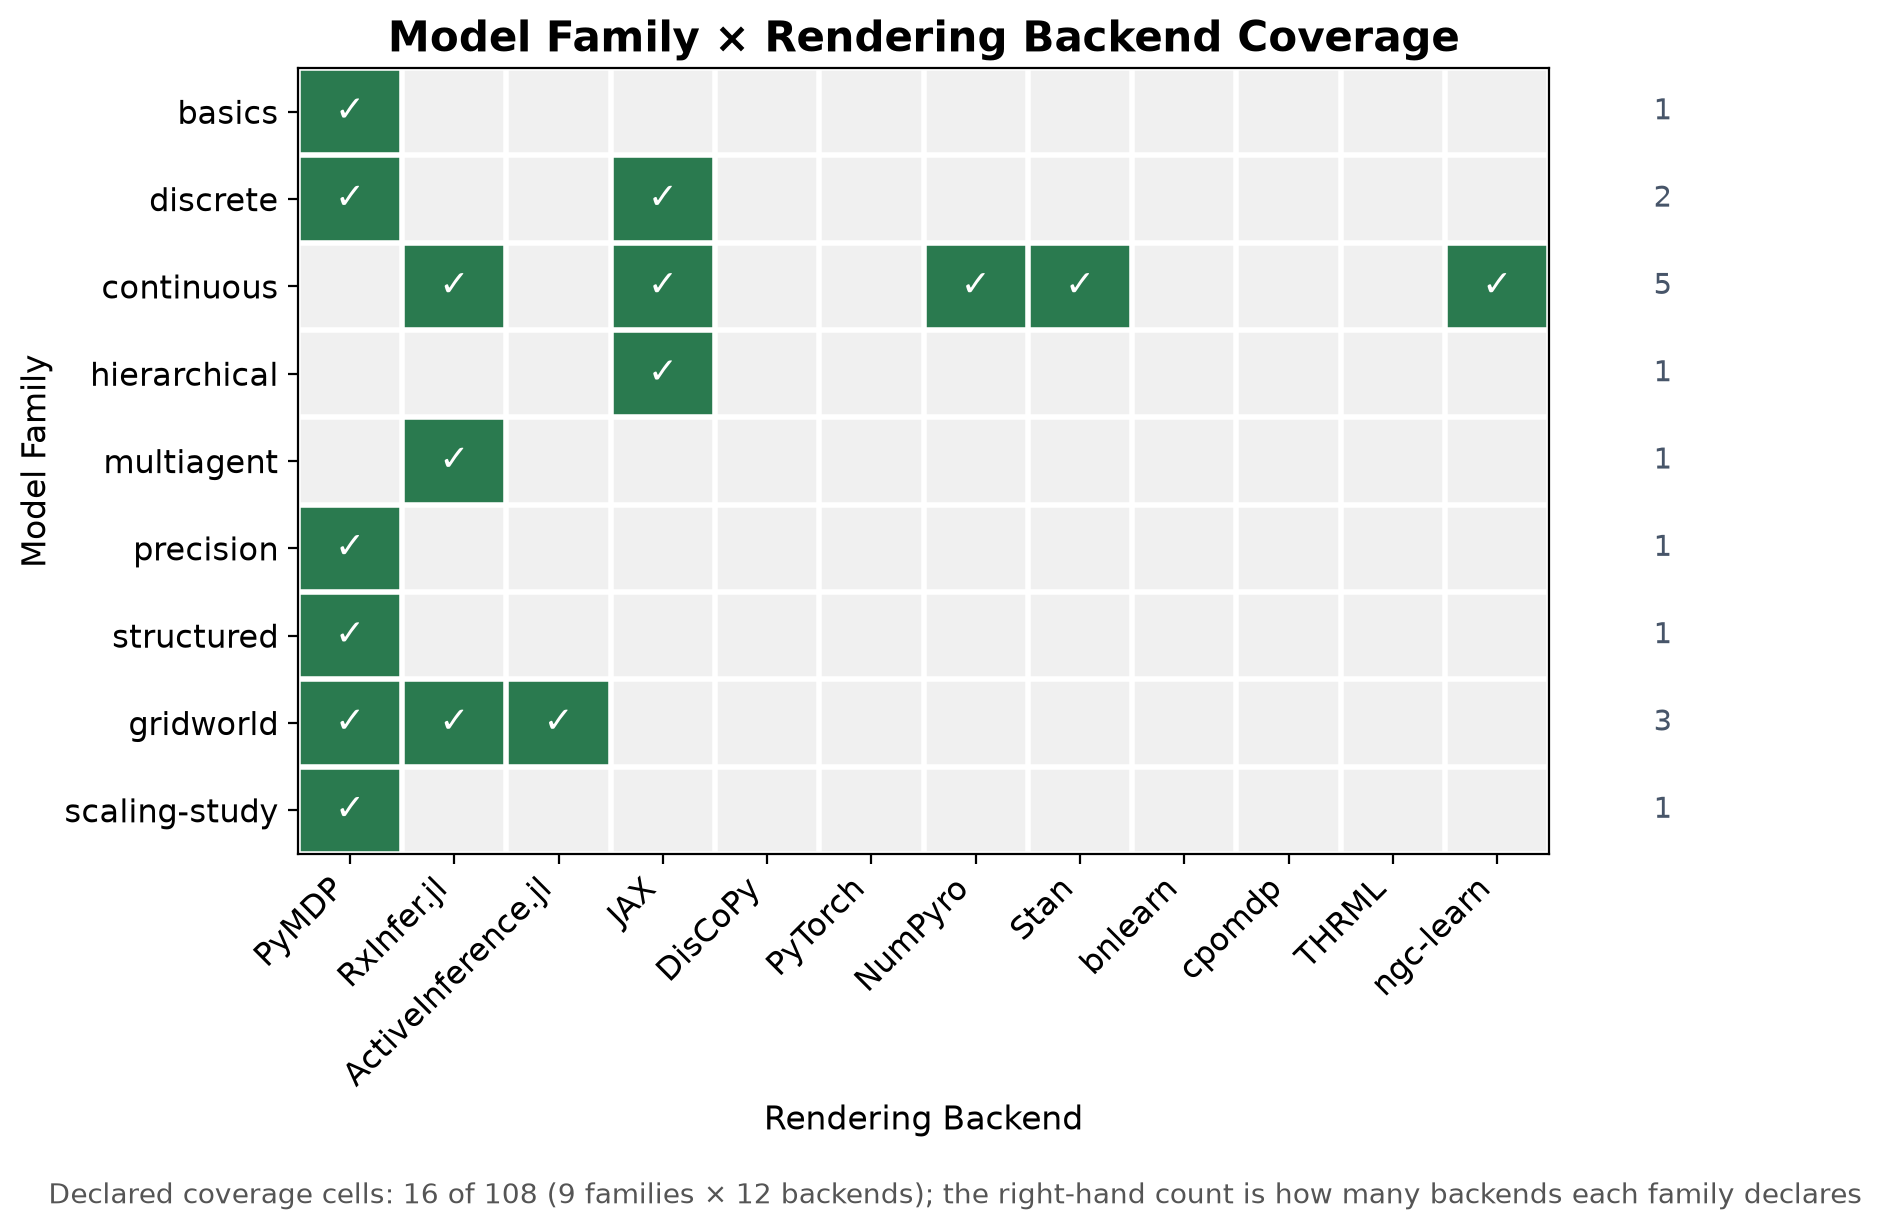
\includegraphics[width=0.85\linewidth,height=0.40\textheight,keepaspectratio,alt={Model-family
coverage across the registered rendering backends: one row per family
from input/model\_family\_manifest.json, one column per backend from
src/gnn/render/framework\_registry.py, and a green cell wherever the
family declares that backend in its frameworks field. The right-hand
count states how many backends each family declares; the grid is
deliberately sparse --- most families declare a single backend, and only
continuous, discrete, and gridworld declare several. Read it as declared
intent, not as profiled outcomes: the gates described below supply the
outcomes. The matrix is generated from the two registries at commit
11a696d6e.}]{../figures/gnn_family_framework_matrix.png}

\end{archiveimageframe}

\end{frame}

\begin{frame}[fragile,allowframebreaks]{Model-Family Coverage}

\begin{archivecaptionframe}

\figurename~6:\ Model-family
coverage across the registered rendering backends: one row per family
from \breaktt{input/model\_family\_manifest.json}, one column per backend
from \breaktt{src/gnn/render/framework\_registry.py}, and a green cell
wherever the family declares that backend in its \texttt{frameworks}
field. The right-hand count states how many backends each family
declares; the grid is deliberately sparse --- most families declare a
single

\end{archivecaptionframe}

\end{frame}

\begin{frame}[fragile,allowframebreaks]{Model-Family Coverage}

\begin{archivecaptionframe}

backend, and only continuous, discrete, and gridworld declare several.
Read it as declared intent, not as profiled outcomes: the gates
described below supply the outcomes. The matrix is generated from the
two registries at commit 11a696d6e.

\end{archivecaptionframe}

\end{frame}

\begin{frame}[fragile,allowframebreaks]{Model-Family Coverage}

These families are not illustrative prose: they are the inputs over
which the parser, the type checker, and the cross-framework code
generators are exercised, and they are the substrate for the reliability
gates described next.
\end{frame}

\begin{frame}[fragile,allowframebreaks]{Semantic-Fidelity and
Cross-Framework Reliability Gates}
\protect\phantomsection\label{semantic-fidelity-and-cross-framework-reliability-gates}
Two command-defined gates check distinct parts of GNN's shared-source
contract on selected family fixtures. Both live under \texttt{scripts/}
and use the family manifest described above. Their actual source-bound
command receipts determine the scope and outcome of verification; the
presence of a gate is not itself a passing result.

The semantic-fidelity gate,
\breaktt{scripts/run\_semantic\_fidelity\_gate.py}, checks
parse--serialize--parse preservation using the versioned
\breaktt{gnn\_semantic\_contract\_v2} contract. It compares model
identity, variables, edges, parameter names, shapes, values and
metadata, equations, timing, and ontology mappings; the default strict
round trip is JSON. Parameter values and their axis order contribute to
the contract hash, so changing values without changing shape changes the
hash. The digest binds the represented contract; it does not prove that
extraction was correct, that generated inference implements the intended
\end{frame}

\begin{frame}[fragile,allowframebreaks]{Semantic-Fidelity and
Cross-Framework Reliability Gates}
mathematics (Da Costa et al. 2020), or that independent numerical
executions agree. The gate reports scoped fidelity per selected model
and format.

A separate numerical witness foundation independently reads a
deliberately restricted source subset without importing the production
parser or renderer. For a small asymmetric categorical model, exhaustive
latent-path enumeration distinguishes filtering on each observation
prefix from smoothing on the complete sequence; actual bnlearn filtering
is compared with the former. For a passive linear-Gaussian model with
rectangular observations, nonzero means and correlated covariances, an
independent joint-Gaussian construction conditions each observation
prefix and is compared with every posterior mean and full covariance
from the generated JAX filter. The first observation uses the declared
prior without an extra prediction. Exact source bytes, variable and axis
\end{frame}

\begin{frame}[fragile,allowframebreaks]{Semantic-Fidelity and
Cross-Framework Reliability Gates}
identities, conditioning horizons, numerical precision and
quantity-specific tolerances remain explicit. Counterexamples change
source identity, orientation, transition/action timing, conditioning,
initial prediction, covariance or precision. These finite, source-bound
comparisons do not establish universal extraction or backend
equivalence, planning correctness or a new Lean proof; formal evidence
remains separately scoped.

The replayable \breaktt{gnn-semantic-witness-v2} receipt retains the
exact source, native result and generated-program bytes together with
the independently reconstructed reference and per-quantity outcomes. The
\texttt{gnn\ witness} interface rebuilds the entire receipt before
accepting a passing numerical outcome; saved arrays or a prior verdict
cannot replace this reconstruction. FEP\_Formal independently replays
the same restricted cases with forward Bayes and recursive Kalman/Joseph
\end{frame}

\begin{frame}[fragile,allowframebreaks]{Semantic-Fidelity and
Cross-Framework Reliability Gates}
updates, using different algorithms from finite path enumeration and
joint-Gaussian conditioning. Separate Lean checks establish
finite-weight normalization and scalar measurement/covariance identities
under their explicit assumptions. These scalar laws are a structural
analogue of the multidimensional Gaussian fixture, not a proof of its
parser, runner or complete translation. Numerical agreement, source
custody, actual program execution and formal compilation remain separate
evidence planes.

\end{frame}

\begin{frame}[fragile,allowframebreaks]{Semantic-Fidelity and
Cross-Framework Reliability Gates}
An additional \breaktt{gnn-semantic-witness-v3} contract admits two
independent stationary passive Gaussian agents. It reconstructs their
authored source independently, builds the joint block-diagonal Gaussian
model and conditions observation prefixes, while retaining complete
native JAX child records and their within-agent covariance matrices. A
separate FEP adapter checks those same authored inputs and native
records with recursive Kalman/Joseph updates. The cross-agent zero
covariance is a consequence of the declared product model, not a
measured native joint covariance. Separate finite post-evidence
product-weight laws and false-claim controls establish their stated
algebraic premises; they do not prove Gaussian conditioning, a parser or
generated execution. Coupling, shared noise, control and unsupported
source or conditioning contracts refuse explicitly.

\end{frame}

\begin{frame}[fragile,allowframebreaks]{Semantic-Fidelity and
Cross-Framework Reliability Gates}
The generated website exposes reported outcomes through offline
status/text filters, posterior and covariance-variance traces, and
residual views, with full tables and raw receipts available alongside
them. Per-agent selectors and full covariance tables expose retained
component results; separate cards show the independent FEP comparisons
and finite compiler controls with their stated scope. Changing a display
control does not rerun a numerical reference or a proof compiler.
Missing or incompatible evidence remains unavailable or refused; an
informative visualization cannot strengthen its underlying scientific
claim.

\end{frame}

\begin{frame}[fragile,allowframebreaks]{Semantic-Fidelity and
Cross-Framework Reliability Gates}
The cross-framework reliability gate,
\breaktt{scripts/run\_cross\_framework\_reliability.py}, takes a single
GNN model and renders it across multiple simulation backends, then
checks that the resulting executable models agree on the structure they
were generated from. The reference comparison runs on the continuous
family across JAX, NumPyro, RxInfer.jl --- 3 independent Active
Inference engines spanning the Python and Julia ecosystems (Heins et al.
2022). The family declares 5 backends (JAX, NumPyro, Stan, RxInfer.jl,
ngc-learn); Stan, ngc-learn is declared but not among the 7 frameworks
the gate profiles, so it is excluded from the comparison. Because the
same source model drives all 3 renderings, source identity helps
investigate disagreement. The gate compares shared matrix shapes, trace
lengths, timesteps, and reported seeds, recording absent comparable
fields separately. These checks do not establish numerical equivalence:
\end{frame}

\begin{frame}[fragile,allowframebreaks]{Semantic-Fidelity and
Cross-Framework Reliability Gates}
a mismatch may arise from extraction, code generation, runtime or
toolchain behavior, inference mode, dtype, or a backend defect.
Numerical comparisons require compatible models and inference semantics,
explicit tolerances, and source-bound numerical witnesses.

Both gates are stated here as commands you can run, not as asserted pass
counts. The manuscript deliberately does not quote a fixed number of
passing checks: an authoritative result is a retained command receipt
bound to its source revision, selected corpus, environment, and
artifacts, and binding a frozen count into prose would invite exactly
the drift the auto-injection contract exists to prevent.

\end{frame}

\begin{frame}[fragile,allowframebreaks]{Semantic-Fidelity and
Cross-Framework Reliability Gates}
A third interchange check extends the same discipline across
repositories: \breaktt{scripts/run\_geo\_interchange\_checks.py}
validates the committed pin in \breaktt{.github/gnn-pair.json} against a
selected GEO-INFER checkout and replays exported GNN artifacts --- the
tracked gridworld, a compiled H3 stay/diffuse model, a rectangular
Gaussian, and an explicit factored fixture --- inside the GEO
environment, writing its receipts even on failure. Like the gates above
it is stated as a command, not as a pass count, and its pinned pair
(\breaktt{ActiveInferenceInstitute/GEO\_INFER} at a recorded revision) is
what makes ``interchange'' a checkable claim rather than a promise.
\end{frame}

\begin{frame}[fragile,allowframebreaks]{Source-Preserving LLM
Processing}
\protect\phantomsection\label{source-preserving-llm-processing}
The LLM analysis step retains exact UTF-8 source parts, task identities,
native responses and resumable checkpoints. Its opt-in
\texttt{joint\_source} mode makes a final request containing the
original source and all ordered fragment answers for each multipart
task; \texttt{part\_evidence} instead supplies derived answers and
source identities. The latter mode does not present the original source
jointly, and neither silently substitutes for the other. Every submitted
source block, task and output reserve must fit the selected model's
context; \texttt{joint\_source} additionally requires the complete
original to fit its final request. Exact source, request, response and
dependency hashes bind cache and resume; incomplete or nonterminal
native outputs remain unfinished.

\end{frame}

\begin{frame}[fragile,allowframebreaks]{Source-Preserving LLM
Processing}
Context admission is limited to reviewed Ollama GGUF runtime contracts.
It binds the exact model digest, advertised and loaded capacity, request
messages, native usage and declared output reserve, with explicit
no-shortening controls and overflow refusal. This is admission under a
reviewed provider contract, not an independent tokenizer or attention
measurement. A retained explicit \texttt{qwen3-coder:30b} profile checks
controlled cross-part fact recovery and a resume with no new
generations; they do not establish general scientific interpretation,
arbitrarily large source coverage or another model's completion quality.
The website presents retained evidence without strengthening those
claims.
\end{frame}

\begin{frame}[fragile,allowframebreaks]{Repository Scale}
\protect\phantomsection\label{repository-scale}
The repository's scale is itself evidence of the surface that the gates
and pipeline cover, and it is reported in fig.~7
directly from the tracked files at commit 11a696d6e.

\end{frame}

\begin{frame}[fragile,allowframebreaks]{Repository Scale}

\refstepcounter{figure}\label{fig:repo_metrics}

\begin{archiveimageframe}

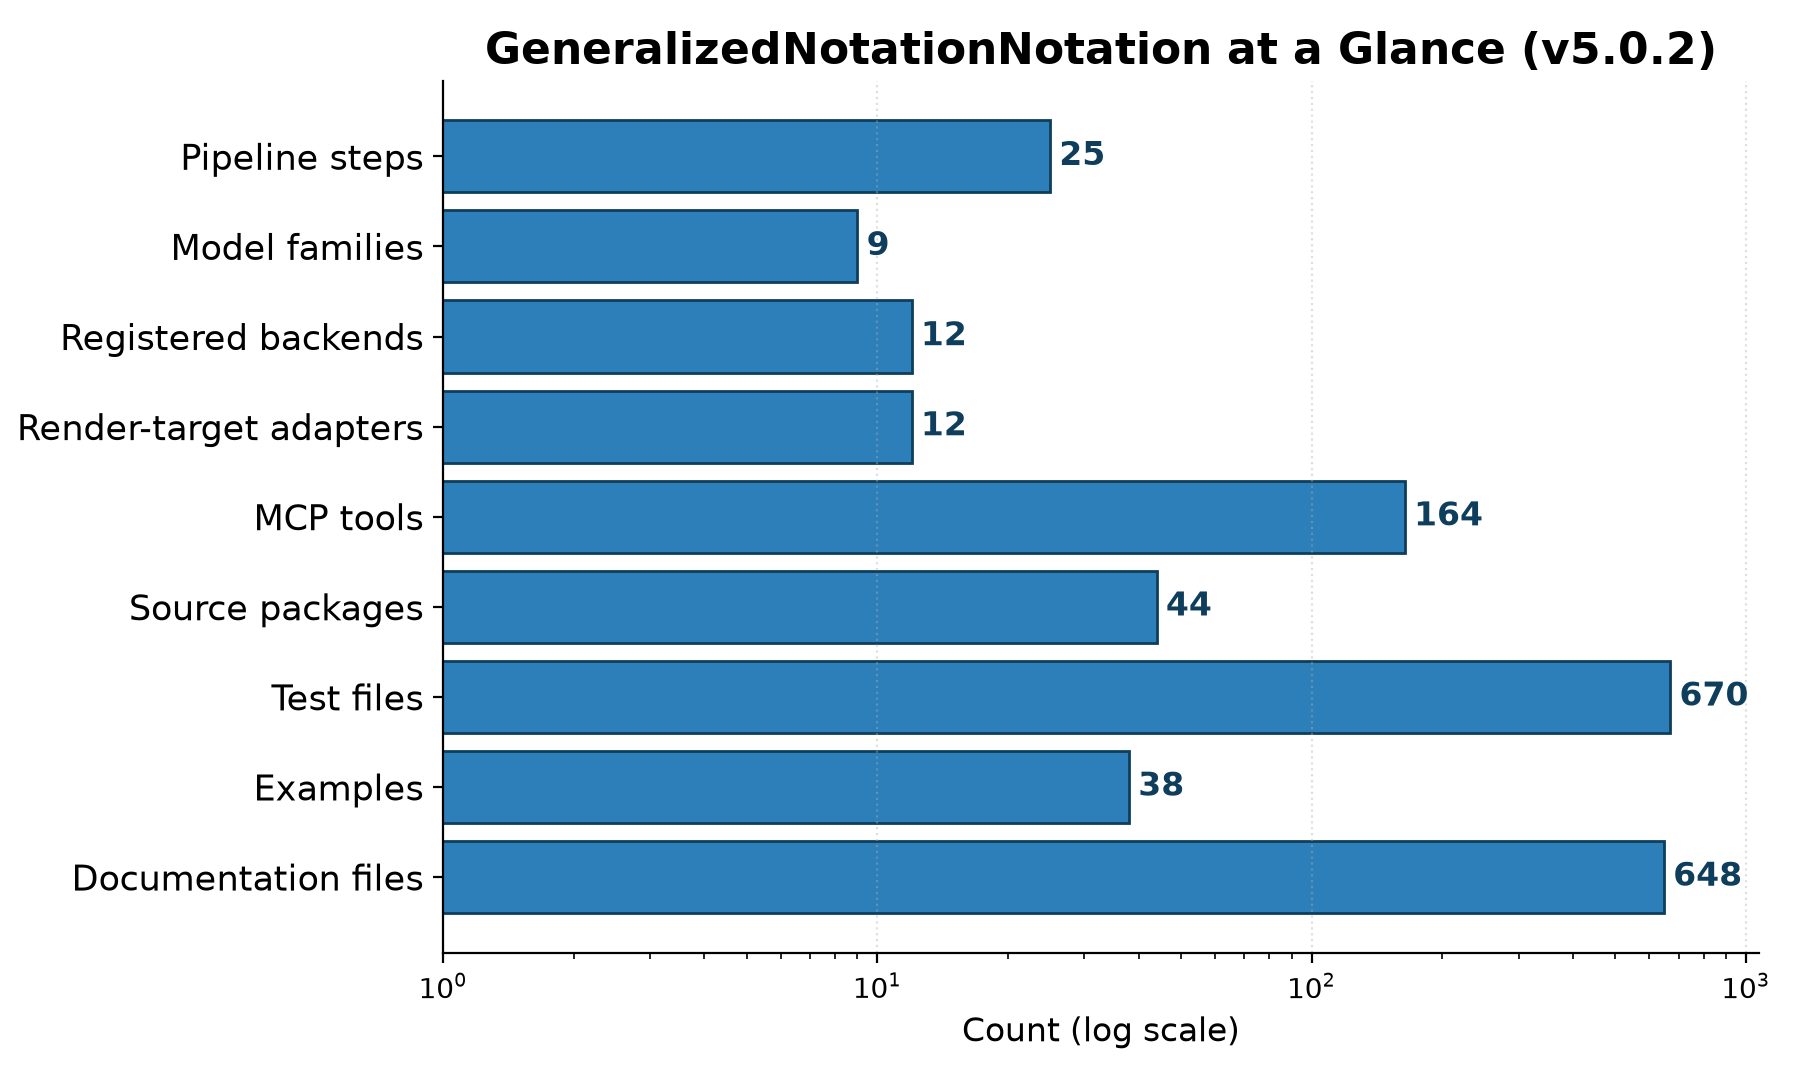
\includegraphics[width=0.8\linewidth,height=0.40\textheight,keepaspectratio,alt={Repository-scale
counts on a logarithmic axis: pipeline steps, model families, registered
backends, render-target execution adapters, Model Context Protocol
tools, source packages, test files, example models, and documentation
files. Every bar is annotated with its exact value, and every value is a
producer token read from output/data/manuscript\_variables.json at
commit 11a696d6e --- the same token map that substitutes the prose
counts. The figure-freshness suite binds the committed image digest and
its recorded producer inputs and counts; semantic content and visual
correctness require their own review. The two backend bars are
deliberately distinct: registered backends (12) counts render targets,
render-target adapters (12) counts the render-target subset with
implemented Step 12 execution adapters. It excludes the separate
execution-only Lean bridge and is not a count of observed native runs.
Read the chart as the scale of the surface the pipeline maintains, not
as a quality measure.}]{../figures/gnn_repo_metrics.png}

\end{archiveimageframe}

\end{frame}

\begin{frame}[fragile,allowframebreaks]{Repository Scale}

\begin{archivecaptionframe}

\figurename~7:\ Repository-scale
counts on a logarithmic axis: pipeline steps, model families, registered
backends, render-target execution adapters, Model Context Protocol
tools, source packages, test files, example models, and documentation
files. Every bar is annotated with its exact value, and every value is a
producer token read from \breaktt{output/data/manuscript\_variables.json}
at commit 11a696d6e --- the same token

\end{archivecaptionframe}

\end{frame}

\begin{frame}[fragile,allowframebreaks]{Repository Scale}

\begin{archivecaptionframe}

map that substitutes the prose counts. The figure-freshness suite binds
the committed image digest and its recorded producer inputs and counts;
semantic content and visual correctness require their own review. The
two backend bars are deliberately distinct: \emph{registered backends}
(12) counts render targets, \emph{render-target adapters} (12) counts
the render-target subset with implemented Step 12 execution

\end{archivecaptionframe}

\end{frame}

\begin{frame}[fragile,allowframebreaks]{Repository Scale}

\begin{archivecaptionframe}

adapters. It excludes the separate execution-only Lean bridge and is not
a count of observed native runs. Read the chart as the scale of the
surface the pipeline maintains, not as a quality measure.

\end{archivecaptionframe}

\end{frame}

\begin{frame}[fragile,allowframebreaks]{Repository Scale}

The test suite comprises 670 test files containing 6943 test functions,
exercising a source base of 776 Python files across 44 packages (231443
lines of source). The pipeline's step modules --- the thin orchestrators
named in tbl.~2 --- number 25, one per numbered
step. The Model Context Protocol surface --- which exposes GNN's
capabilities to external agents and tools --- provides 164 tools across
36 modules. The pipeline itself runs as 25 steps (0--24), and 7 figure
artifacts from the rendering of figures, models, and reports are
committed under \texttt{output/}, of which 7 are the manuscript's own.
\end{frame}

\begin{frame}[fragile,allowframebreaks]{Claim Discipline}
\protect\phantomsection\label{claim-discipline}
A claim is manuscript-ready only when it is bound to a verifiable
artifact. Concretely, every claim in this manuscript must rest on one of
four support types:

\end{frame}

\begin{frame}[fragile,allowframebreaks]{Claim Discipline}
\begin{itemize}
\tightlist
\item
  A retained passing test or validator command receipt, bound to the
  source revision, selected inputs, environment, and artifacts --- for
  example a scoped execution of the semantic-fidelity or cross-framework
  gates above.
\item
  A generated output produced by a deterministic producer, such as the
  figures rendered from the family and repository scans, or the token
  values emitted by the manuscript-variable producer that backs every
  number on this page.
\item
  A source ledger, manifest, or configuration file that fixes a declared
  value or capability; actual execution still requires its own result
  receipt.
\item
  A resolved entry in \texttt{references.bib} for any
  external-literature claim (Friston 2010; Parr et al. 2022).
\end{itemize}

\end{frame}

\begin{frame}[fragile,allowframebreaks]{Claim Discipline}
The pipeline records its own evidence trail under \texttt{output/}. The
run-level summary is written to \breaktt{output/PIPELINE\_REPORT.md}, and
the per-step execution record --- including which steps ran, their
status, and their artifacts --- is captured in
\breaktt{output/00\_pipeline\_summary}. Readers should use those
current-run records and their identity bindings to assess actual
pipeline outcomes. Repository counts and declared capability tokens
describe the source surface and do not by themselves establish native
execution or scientific correctness. When a value would otherwise need a
literal number with no producer behind it, the discipline is to omit the
number rather than to hard-code it.
\end{frame}

\end{document}
